\documentclass{../../ece-report}

\usepackage{subcaption}
\usepackage{multirow}


\memostudent{Ty Davis}
\memotitle{Lab 5 - DC biasing of an NMOS transistor}
\memocourse{ECE 3110}
\memodate{\today}


\newcommand{\Vsub}[1]{\ensuremath{\textnormal{V}_{#1}}}
\newcommand{\sub}[2]{\ensuremath{\textnormal{#1}_{#2}}}

\renewcommand{\half}{\frac{1}{2}}



\begin{document}

\maketitle


\section{Introduction and Theory}

In Fig.~\ref{fig:circuit} you can see the circuit that
we used in the lab. We are going to use this circuit
to force the NMOS transistor into both the triode and
saturation regions. To do that we will need to select
certain resistors to cause the voltages at $\textnormal{V}_{D}$, \Vsub{G},
and \Vsub{S} to reach specific levels that suggest triode
and saturation operation of the MOSFET. In order to
verify our calculations we will simulate and build/measure
the circuit to compare to our analysis.

\begin{figure}[h!]
  \centering
  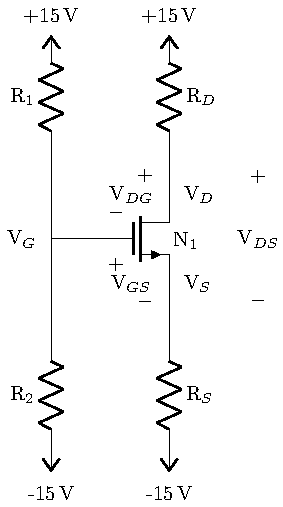
\includegraphics{circuits/circuit.pdf}
  \caption{Circuit that we use in the lab.}\label{fig:circuit}
\end{figure}

\section{Saturation Region}

The saturation region is characterized by $\Vsub{DS} >
v_{ov}$, and we've been asked to design the circuit
such that $\sub{I}{D}=1~\si{\mA}$, $\Vsub{G}=0~\si{\V}$, and $\Vsub{D}=5~\si{\V}$.

\subsection{Calculations}

\subsubsection{Find \sub{R}{D}}

Because \sub{I}{D} and \Vsub{D} are provided, \sub{R}{D} is easy to find: 

$$\sub{R}{D}=\frac{\Vsub{DD}-\Vsub_{D}}{\sub{I}{D}} = \frac{15 - 5}{0.001} = 10~\si{\kohm}$$

\subsubsection{Find \sub{R}{S}}

Calculating \sub{R}{S} is a little bit more involved.
First we need to find \Vsub{S}, but to do that we need
to find \Vsub{GS}. In the saturation region we know

\[
  \sub{I}{D}=\half k_n (\Vsub{GS} - \Vsub{th}) ^ 2
\]

This can be rearranged to solve for \Vsub{GS}, and we get Eq.~\ref{eq:v_gs}

\begin{equation}
  \Vsub{GS} = \sqrt{\frac{2 \cdot \sub{I}{D}}{k_n}} + \Vsub{th}
  \label{eq:v_gs}
\end{equation}

From the datasheet we can find an operating point which
we can use to calculate $k_n$ using 

\[
  k_n = \frac{1}{\sub{r}{DS} \cdot \sub{v}{OV}} 
\]

In the datasheet we read that $\Vsub{th} = 2.15~\si{\V}$, and
we get the operating point $\sub{r}{DS} = 1.8~\si{\ohm}$ @ $\Vsub{GS} = 10~\si{\V}$.
Thus, we can get $k_n$:

\[
  k_n = \frac{1}{1.8 \cdot 7.9} = 0.070~\si{\A/\V^2}
\]

Using that $k_n$ we can obtain \Vsub{GS}:

\[
  \Vsub{GS} = \sqrt{\frac{2 \cdot 1~\si{\mA}}{0.2462~\si{A}/\si{V}^2}} + 2.15~\si{\V}= 2.269~\si{\V} 
\]

Finally, we know that $\Vsub{S} = \Vsub{G} - \Vsub{GS} = -2.269~\si{\V}$. And using $\Vsub{S} = -2.269~\si{\V}$ we can
calculate \sub{R}{S}.

$$\sub{R}{S}=\frac{\Vsub{S} - \Vsub{SS}}{\sub{I}{D}} = \frac{-2.269 - (-15)}{0.001} = 12.731 \si{\kohm}$$.

\subsubsection{Find \sub{R}{1} and \sub{R}{2}}

Finally, to calculate \sub{R}{1} and \sub{R}{2} we need
to ensure that the voltage $\Vsub{G} = 0~\si{\V}$. With
only one current path, that means that we want to select
any two equal value resistors. The problem is not completely
defined and we can pick any that we want, though we
will likely want to pick some high-value resistors to
keep the current flow low and use less power. We can
use $\sub{R}{1}=\sub{R}{2}=1~\si{\Mohm}$.

\subsection{Simulation}

With the calculated values from the previous section, we were able to 
simulate the circuit and we got these values.

\begin{table}[h!]
  \centering
  \begin{tabular}{c c c c}\toprule
    \textbf{\Vsub{D}} & \textbf{\Vsub{S}} & \textbf{\Vsub{G}} & \textbf{\sub{I}{D}} \\
    4.90~V & -2.14 V & 0 V & 1.01 mA \\
    \bottomrule
  \end{tabular}
  \caption{Simulation results in saturation.}
  \label{tab:sim_sat}
\end{table}

The differences between the simulation and our calculations
were present but very minimal, all within 0.1~V and 10~\si{\uA}.

\subsection{Measurements}

To build the circuit we needed to select the right resistors,
but without those precise resistors in the lab we need to build
equivalent resistor networks from the available resistors. All of the 
used resistors values are shown in Table~\ref{tab:res_sat}.

\begin{table}[h!]
  \centering
  \begin{tabular}{l c c c}\toprule
    & \textbf{Calculated Resistor} & \textbf{Equivalent Resistor} & \textbf{Measured Resistor} \\
    \midrule
    \multirow{4}{*}{\sub{R}{S}} & 12.731 \si{\kohm} & 12.670 \si{\kohm} & 12.595 \si{\kohm} \\
               & --- & 2.2 \si{\kohm} & 2.181 \si{\kohm} \\
               & --- & 10 \si{\kohm} & 9.949 \si{\kohm} \\
               & --- & 470 \si{\kohm} & 0.465 \si{\kohm} \\
    \midrule
    \sub{R}{D} & 10 \si{\kohm} & 10 \si{\kohm} & 9.875 \si{\kohm} \\
    \midrule
    \sub{R}{1} & 1 \si{\Mohm} & 1 \si{\Mohm} & 0.968 \si{\Mohm} \\
    \midrule
    \sub{R}{2} & 1 \si{\Mohm} & 1 \si{\Mohm} & 0.983 \si{\Mohm} \\

    \bottomrule
  \end{tabular}
  \caption{Resistors used to operate in saturation region.}
  \label{tab:res_sat}
\end{table}


\begin{table}[h!]
  \centering
  \begin{tabular}{c c c c}\toprule
    \textbf{\Vsub{D}} & \textbf{\Vsub{S}} & \textbf{\Vsub{G}} & \textbf{\sub{I}{D} (calculated)} \\
    4.831~V & -2.04 V & 0.116 V & 1.03 mA \\
    \bottomrule
  \end{tabular}
  \caption{Measurement results in saturation region.}
  \label{tab:meas_sat}
\end{table}

\section{Triode Region}

Now we are tasked with designing the same circuit such
that the MOSFET is operating in the triode region. We
need to obtain the following parameters: $\sub{I}{D}=
10~\si{\mA}$, $\sub{V}{D}=2~\si{\V}$, and $\Vsub{DS}=0.1~\si{\V}$

\subsection{Calculations}

\subsubsection{Find \sub{R}{D}}

Once again, finding \sub{R}{D} is trivial:

\[
  \sub{R}{D}=\frac{\Vsub{DD}-\Vsub_{D}}{\sub{I}{D}} = \frac{15 - 2}{0.01} = 1.3~\si{\kohm}
\]

\subsubsection{Find \sub{R}{S}}

Finding \sub{R}{S} is easy this time because we know
that $\Vsub{S} = \Vsub{D} - 0.1 = 1.9~\si{\V}$.

So:

\[
  \sub{R}{S} = \frac{\Vsub{S} - \Vsub{SS}}{\sub{I}{D}} = \frac{1.9 - (-15)}{0.01} = 1.69~\si{\kohm}
\]


\subsubsection{Find \sub{R}{1} and \sub{R}{2}}

This time finding \sub{R}{1} and \sub{R}{2} is a bit
more difficult. We don't know \Vsub{G}, but we can find
it if we know \Vsub{GS} because we already know \Vsub{S}.

\[
  \sub{I}{D} = k_n \Big(\sub{v}{OV} - \half \Vsub{DS} \Big) \Vsub{DS}
\]

Substituting $\sub{v}{OV} = \Vsub{GS} - \Vsub{th}$,
and distributing the \Vsub{DS} in we get this polynomial
equation:

\[
  \sub{I}{D} = k_n \Big((\Vsub{GS} - \Vsub{th})\Vsub{DS} - \half \Vsub{DS}^2 \Big)
\]

Using the values that we know from the problem description, and the $k_n$ that we calculated in the last section, we get

\[
  10~\si{\mA} = 0.070 \Big( (\Vsub{GS}-2.1)\cdot 0.1 - \half (0.1)^2 \Big)
\]

Solving for \Vsub{GS} yields $\Vsub{GS} = 3.579~\si{\V}$.

Knowing that $\Vsub{S} = 2 - 0.1 = 1.9 \si{\V}$, we
can obtain $\Vsub{G} = \Vsub{GS} + \Vsub{S} = 5.679
\si{\V}$.

With $\Vsub{G} = 5.679~\si{\V}$, we can determine the voltage divider that
we want for \sub{R}{1} and \sub{R}{2}. Keeping \sub{R}{2} at 1~\si{\Mohm}, we 
can find that $\sub{R}{1}=0.4649~\si{\Mohm}$.

\subsection{Simulation}

We designed the circuit in Multisim and the results are shown in Table~\ref{tab:sim_triode}.

\begin{table}[h!]
  \centering
  \begin{tabular}{c c c c}\toprule
    \textbf{\Vsub{D}} & \textbf{\Vsub{S}} & \textbf{\Vsub{G}} & \textbf{\sub{I}{D}} \\
    1.99~V & 1.91 V & 5.48 V & 10.0 mA \\
    \bottomrule
  \end{tabular}
  \caption{Simulation results in triode.}
  \label{tab:sim_triode}
\end{table}

Once again, the voltages are all right in line with
our calculations, with only a little bit of variation.

\subsection{Measurements}


A similar process was done to select the resistors.
They are shown in Table~\ref{tab:res_triode}.


\begin{table}[h!]
  \centering
  \begin{tabular}{l c c c}\toprule
    & \textbf{Calculated Resistor} & \textbf{Equivalent Resistor} & \textbf{Measured Resistor} \\
    \midrule
    \multirow{3}{*}{\sub{R}{S}} & 1690 \si{\ohm} & 1680 \si{\ohm} & 1657 \si{\ohm} \\
               & --- & 1000 \si{\ohm} & 987 \si{\ohm} \\
               & --- & 680 \si{\ohm} & 670 \si{\ohm} \\
    \midrule
    \multirow{4}{*}{\sub{R}{D}} & 1300 \si{\ohm} & 1304 \si{\ohm} & 1287 \si{\kohm} \\
          & --- & 68 \si{\kohm} & 67.32 \si{\kohm} \\
          & --- & 330 \si{\ohm} & 328 \si{\ohm} \\
          & --- & 1 \si{\kohm} & 0.985 \si{\kohm} \\
    \midrule
    \sub{R}{1} & 0.465 \si{\Mohm} & 0.470 \si{\Mohm} & 0.465 \si{\Mohm} \\
    \midrule
    \sub{R}{2} & 1 \si{\Mohm} & 1 \si{\Mohm} & 0.983 \si{\Mohm} \\

    \bottomrule
  \end{tabular}
  \caption{Resistors used to operate in triode region.}
  \label{tab:res_triode}
\end{table}


\begin{table}[h!]
  \centering
  \begin{tabular}{c c c c}\toprule
    \textbf{\Vsub{D}} & \textbf{\Vsub{S}} & \textbf{\Vsub{G}} & \textbf{\sub{I}{D} (calculated)} \\
    1.889~V & 1.861 V & 5.193 V & 10.2 mA \\
    \bottomrule
  \end{tabular}
  \caption{Measurement results in triode region.}
  \label{tab:meas_triode}
\end{table}

This time, there was a bit more discrepancy between the calculated values
and our measured ones, but the difference remains small. As such, it is safe
to assume that the device is operating as expected.

\section{Conclusion/Post Lab Observations}

When building the the circuit that was designed for
saturation operation, we got the values of $\Vsub{GS}=2.156~\si{\V}$
and $\Vsub{DS}=6.871~\si{\V}$. These values clearly
suggest that the device is operating in the saturation
region because $\Vsub{DS} > \sub{v}{OV}$, and \sub{v}{OV}
is incredibly close to 0.

After building the circuit to operate in the triode region,
we found $\Vsub{GS}=3.332~\si{\V}$ and $\Vsub{DS} = 0.028~\si{\V}$.
These show that the device is operating in the triode region because
$\Vsub{DS} < \sub{v}{OV}$. $\sub{v}{OV}\approx 1.1~\si{\V}$. 


The currents that we got for \sub{I}{D} when we built
the circuits for saturation and triode operation are
also right in line with the calculation. They are shown
in the corresponding measurement tables.


\end{document}
